A functional parameterization of a problem is called an \emph{ansatz}. 
Not every ansatz is able to represent every wavefunction and some are way more efficient in the amount of necessary trainable parameters than others.

Even if the metaformer architecture is already chosen as an ansatz, there are still multiple different possibilities to output the final value for the wavefunction.

It is common knowledge that the quantum mechanical wavefunction is a function that maps into the complex domain.
Though some problems require a complex valued wavefunction (this for example is very common for \emph{time-dynamic} problems, but here only \emph{static} wavefunctions are calculated), it can also be sufficient to have a completely real valued one.
If the real part of the wavefunction is sufficient, it is obviously not helpful to dedicate resources to the imaginary part.

\autoref{fig:ansatz-comparisons} shows the four possible choices of ansatz implemented in the accompanying code.
Of the four network architectures, three of them are entirely real-valued (sr, tr and spc). 
The forth one (sc) is a \emph{complex valued network} \cite{deepComplexNetworks}.
The sc network ansatz will not be shown in later lineups. 
Because of its complex weights, every number requires the double the amount of memory (equal precision storage of real  and imaginary part). 
Also the multiplication of complex numbers requires more operations to perform.
Both of these facts make the training and evaluation of the network slower. 
Not only require more weights most of the time a bigger number of backpropagation steps, but also the time per step is stretched. 
Overall making the sc ansatz too expensive to compute in this application.

The ansatz with the real output and the two versions with the assembled complex output are measured for their rate of convergence in \autoref{fig:hyperparameter-matrix}.
It can be noted, that the selected metaformer \emph{hyperparameters} (\autoref{sec:experiments-hyperparameters}) influence the most and least efficient ansatz.
No one ansatz can be pointed out as the best suited one, not even for a fixed lattice problem.

This once again underlines the flexibility that comes with the presented metaformer framework, but stresses the requirement for intensive testing to be able to choose the most appropriate architecture.

\begin{figure}[htbp]
    \centering
    \makebox[\textwidth][c]{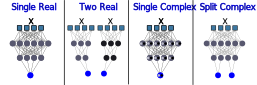
\includegraphics[width=1\textwidth]{./experiments/ground-state-search/ansatz/ansatz.pdf}}
    \caption{
        Schematic visualization of how the four different possibilities for the ansatz are implemented.
        \emph{Single Real} gives a pure real wavefunction output. The architecture is a single network with only real parameters.
        \emph{Two Real} gives a complex wavefunction output (two real numbers, one for the phase and one for the amplitude). The architecture consists of two half-size networks with only real parameters. They do not interact.
        \emph{Single Complex} gives a complex wavefunction output (directly one complex type number). The architecture is a single network with every parameter being a complex number.
        \emph{Split Complex} gives a complex wavefunction output (two real numbers, one for the phase and one for the amplitude). The architecture is a single network with only real parameters, but at the last stage it is split to give two outputs instead of one. The difference to the two real ansatz is that the two \glqq halves\grqq{} of the network can interact.
    }
    \label{fig:ansatz-comparisons}
    
    \makebox[\textwidth][c]{\includegraphics[width=1.1\textwidth]{./experiments/ground-state-search/ansatz/hyperparameter-matrix/hyperparameter-matrix.pdf}}
    \caption{Comparison of hyperparameter combinations. 
            The ansatz is encoded in the dash type, the color specifies the metaformer hyperparameters.
            \emph{sr d:1 e:8} meaning \emph{single real}, \emph{depth 1} and \emph{embed dimension 8}.
            All datasets have been calculated for a randomly encoded \emph{trigonal\_square} lattice with 64 lattice sites.
            Every model is of the type \emph{GPF-NNN} with a mlp-ratio of 4. The Ising parameters are $J=-1$ and $h=-0.7$.
    }
    \label{fig:hyperparameter-matrix}
\end{figure}
